%%%%%%%%%%%%%%%%%%%% author.tex %%%%%%%%%%%%%%%%%%%%%%%%%%%%%%%%%%%
%
% sample root file for your "contribution" to a proceedings volume
%
% Use this file as a template for your own input.
%
%%%%%%%%%%%%%%%% Springer %%%%%%%%%%%%%%%%%%%%%%%%%%%%%%%%%%


\documentclass[12pt]{svproc}
\usepackage{graphicx}
\graphicspath{ {/figures/} }
\usepackage{url}
\usepackage[export]{adjustbox}
\usepackage{subcaption}
\captionsetup{compatibility=false}
\usepackage[utf8]{inputenc}
\usepackage{wrapfig}
\usepackage{amsmath}
\usepackage{amssymb}
\usepackage{minted}
\usepackage{inputenc}
\usepackage{listings}
\usepackage{color}
 
\definecolor{codegreen}{rgb}{0,0.6,0}
\definecolor{codegray}{rgb}{0.5,0.5,0.5}
\definecolor{codepurple}{rgb}{0.58,0,0.82}
\definecolor{backcolour}{rgb}{0.95,0.95,0.92}
 
\lstdefinestyle{mystyle}{
    backgroundcolor=\color{backcolour},   
    commentstyle=\color{codegreen},
    keywordstyle=\color{magenta},
    numberstyle=\tiny\color{codegray},
    stringstyle=\color{codepurple},
    basicstyle=\footnotesize,
    breakatwhitespace=false,         
    breaklines=true,                 
    captionpos=b,                    
    keepspaces=true,                 
    numbers=left,                    
    numbersep=5pt,                  
    showspaces=false,                
    showstringspaces=false,
    showtabs=false,                  
    tabsize=2
}
 
\lstset{style=mystyle}

\usepackage[left=1in,right=1in,top=1in,bottom=1in,footskip=0.25in]{geometry}


\def\UrlFont{\rmfamily}

\begin{document}
	


\title{NBR Mapping using Google Earth Engine}

%
\author{}
\institute{By Vanshika Gupta(16CV245)\\Seminar Report(CV390)\\National Institute of Technology Karnataka, Surathkal\\~\\ 
Guided by Ms.Amba Shetty \\
Department of Applied Mechanics and Hydraulics\\
National Institute of Technology Karnataka, Surathkal\\
}


\maketitle              % typeset the title of the contribution
%

\section{\Large Abstract}
The Objective of the seminar was to illustrate the use of Google Earth Engine to map the Normalised Burnt Ratio(NBR) and the Difference normalised burnt ratio(dNBR) for dataset of the Bandipur and the KM park project in the North Karnataka region. By using Google earth engine, we automate the procedure of importing the dataset, code up the algorithm involved and finally map the NBR. After mapping, we analysed the results using fire points data available.

\section[60pt]{\Large Introduction}
%

\subsection{Google Earth Engine}
The Google Earth Engine (GEE) platform contains petabyte-scale data for scientific analysis and visualization. After the Landsat image series were made freely available in 2008, Google consolidated this very large and useful data set and linked it to its cloud computing resources to make available to the scientific community one of the largest datasets for studying the earth’s resources. GEE now includes satellite datasets from a number of other platforms, as well as many vector-based datasets.\\

The easily accessible and user-friendly front-end provides a convenient environment for interactive data and algorithm development. Users are also able to add and curate their own data and collections, while using Google’s cloud resources to undertake all the processing. The end result is that this now allows scientists, independent researchers, hobbyists and nations to mine this massive warehouse of data for change detection, map trends and quantify resources on the Earth's surface like never before. One does not need large processing powers of the latest computers or the latest software, meaning that resource poor researchers in the poorest nations of the world have the same ability to undertake analysis as those in the most advanced nations.\\

Applications of GEE include, but are not limited to: mapping forest cover, detecting deforestation, classifying land cover, estimating forest biomass and carbon, mapping urban area expansion, population mapping, changes in agricultural production and forecasting, and rangeland dynamics.\\

This collection calls for example applications of GEE all over the world and in all disciplines. We particularly encourage articles from developing nations on how the availability of GEE data and processing has enabled new research that was difficult or impossible before. We also encourage papers on issues about using GEE, processing shortcomings, programming, and difficulties in handling data in the cloud atmosphere. Anything to do with GEE is suitable for this collection.\\

The Earth Engine API is available in Python and JavaScript, making it easy to harness the power of Google’s cloud for your own geospatial analysis. \\

\subsection{Normalised Burnt Ratio}
The Normalized Burn Ratio (NBR) was designed to highlight burned areas and estimate fire severity. The formula is similar to NDVI, except that it uses near-infrared (NIR) and shortwave-infrared (SWIR) wavelengths.\\

 \begin{equation}
NBR = \frac{NIR - SWIR}{NIR + SWIR}
\end{equation}
 \graphicspath{ {./figures/} }
 
 Pre-fire, healthy vegetation has very high near-infrared reflectance and low reflectance in the shortwave infrared portion of the spectrum. Recently burned areas on the other hand have relatively low reflectance in the near-infrared and high reflectance in the shortwave infrared band. A high NBR value generally indicates healthy vegetation while a low value indicates bare ground and recently burned areas.\\
 
 	\begin{figure}{}
 		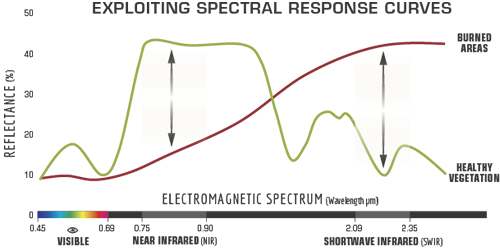
\includegraphics[width=0.9\linewidth, height=5cm]{p1.png} 
 		%\caption{Caption1}
 		\label{fig:subim1}
 		\centering
 		 	\caption{Image Credit: US Forest Servicel}
 	\end{figure}
 
 \subsection{Burnt Severity}
Normalized Burn Ratio is frequently used to estimate burn severity. Imagery collected before a fire will have very high near infrared band values and very low mid infrared band values and a Imagery collected over a forest after a fire will have very low near infrared band values and very high mid infrared band values. Higher dNBR indicate more severe damage. Areas with negative dNBR values may indicate increased vegetation productivity following a fire.\\
 
 \begin{equation}
dNBR (or) \Delta NBR  = PrefireNBR - PostfireNBR
\end{equation}	\\


The meaning of the ∆NBR values can vary by scene, and for best results interpretation in specific instances should always be based on some field assessment. However, the adjacent table from the USGS FireMon program can be useful as a first approximation for interpreting the NBR difference. These guidelines are then used to create a thematic burn severity layer depicting severity as unburned to low, low, moderate, high, and increased greenness (increased post-fire vegetation response).\\

Typically, $NBR$ and $\Delta NBR$ images are generated shortly after a fire burns to get an initial assessment of burn severity and to support field work. During the next growing season, NBR datasets are often calculated again to assess vegetation survival and delayed mortality. Burn severity data and maps can aid in developing emergency rehabilitation and restoration plan post-fire. They can be used to estimate soil burn severity and to estimate the likely future downstream impacts due to flooding, landslides, and soil erosion. \\

\begin{figure}{}
	\fbox{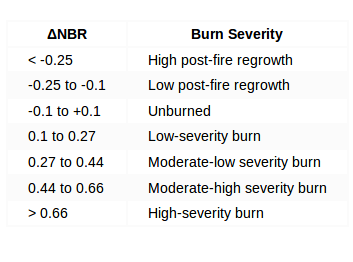
\includegraphics[width=0.7\linewidth, height=7cm]{p2.png} }
	%\caption{Caption1}
	\label{fig:subim1}
	\centering
	\caption{Classification based on NBR values}
\end{figure}

 When uses indices as part of an analysis it is important to make sure data has been appropriately preprocessed. This usually involves radiometric calibration and atmospheric correction. To get the most information out of a spectral index it is optimal to collect ground truth data to calibrate and validate the index.

\section{Dataset}
\subsection{Satellite Data}

We tried the following procedure for 2 satellite datas and two datasets
\begin{itemize}
	\item Sentinel-2 MSI: MultiSpectral Instrument, Level-1C \\ \\This is a wide-swath, high-resolution, multi-spectral imaging mission supporting Copernicus Land Monitoring studies, including the monitoring of vegetation, soil and water cover, as well as observation of inland waterways and coastal areas.\\ \\ The Sentinel-2 data contain 13 UINT16 spectral bands representing TOA reflectance scaled by 10000. In addition, three QA bands are present where one (QA60) is a bitmask band with cloud mask information.\\
	
	\begin{figure}{}
	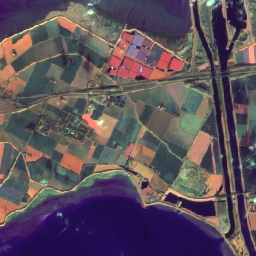
\includegraphics[width=0.5\linewidth, height=7cm]{p5.png} 
	%\caption{Caption1}
	\label{fig:subim1}
	\centering
	\caption{Landsat 8 Image}
    \end{figure}
	
	\item USGS Landsat 8 Surface Reflectance Tier 1 \\ \\
	This dataset is the atmospherically corrected surface reflectance from the Landsat 8 OLI/TIRS sensors. These images contain 5 visible and near-infrared (VNIR) bands and 2 short-wave infrared (SWIR) bands processed to orthorectified surface reflectance, and two thermal infrared (TIR) bands processed to orthorectified brightness temperature.\\ \\ These data have been atmospherically corrected using LaSRC and includes a cloud, shadow, water and snow mask produced using CFMASK, as well as a per-pixel saturation mask. Strips of collected data are packaged into overlapping "scenes" covering approximately 170km x 183km using a standardized reference grid.
\end{itemize}

\begin{figure}{}
	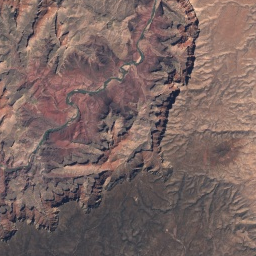
\includegraphics[width=0.5\linewidth, height=7cm]{p4.png} 
	%\caption{Caption1}
	\label{fig:subim1}
	\centering
	\caption{Landsat 8 Image}
\end{figure}

\subsection{Locations}
 \subsubsection{Bandipur}
 
 On 21 February 2019, wildfire broke out in the Bandipur Tiger Reserve. Unlike in previous years, this is the first time the wildfire in Bandipur flared up earlier due to the sudden climatic change and rapid growth of dry grass and Lantana. Officials reported that there appeared to have been no deaths of the larger mammals in the Park, such as bison, elephants, leopard and tiger.\\

Over 10,000 acres of forest in Bandipur area was destroyed. With the fire spreading rapidly due to winds, the authorities closed the Gundlupet-Ooty National highway and safaris in Bandipur National Park were also cancelled. Strong winds were making the job of firefighters, forest staff and volunteers more difficult.\\

The fire that destroyed Kundakere Range, spread to Barakatte and Guddakere, then to the Himavathi Gopalaswamy Hills. It also destroyed forests in Jarkal Kere and Gowri Kalu hills. Many smaller mammals and reptiles were killed, along with thousands of trees.There had been no forest-fire incidents noted in Bandipur National Park in the previous two years.[7] \\

\begin{figure}{}
	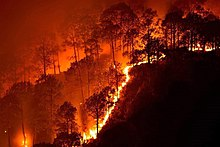
\includegraphics[width=0.7\linewidth, height=7cm]{p3.jpg} 
	%\caption{Caption1}
	\label{fig:subim1}
	\centering
	\caption{Bandipur Fire}
\end{figure}

%  MATLAB Code for creating synthetic image \\
%  \hline
%  \inputminted{octave}{createImage.m}
%  \hline
%  \vspace{0.5cm}
%  Code for dirichlet sampling distribution:\\
%  \hline
%  \inputminted{octave}{dirichletSampling.m}
% \hline


\section{Methodology}
%
\subsection{Opening and running code in the Code Editor}
The steps below demonstrate how to open Earth Engine and execute a custom script that displays an image.

\begin{itemize}
	\item Open the Earth Engine Code Editor here: code.earthengine.google.com. If you have not already, you will need to enable access by logging in using a registered Google account.\\
	\item Navigate to the Scripts tab located on the far left of the Code Editor. There you will find a collection of example scripts that access, display, and analyze Earth Engine data.\\
	\item Under “Image Collection,” select the “Filtered Composite” example. You will see a script appear in the center console. Press the Run button to execute the script. The Filtered Composite example selects Landsat 7 images that intersect or are within the boundaries of Colorado and Utah. It then displays a true color composite of the selected images. The samples introduce you to commonly used methods, such as filter(), clip(), and Map.addLayer().
\end{itemize}

 \begin{figure}{}
	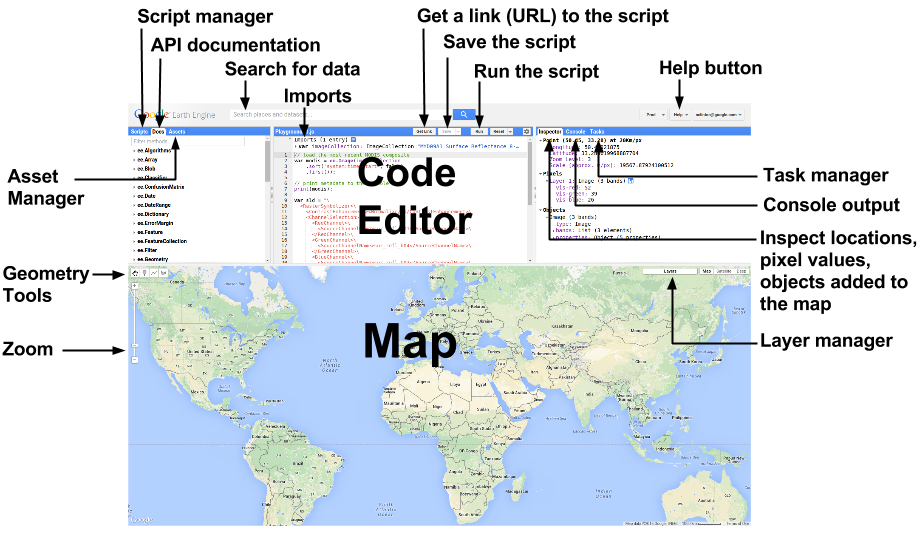
\includegraphics[width=0.7\linewidth, height=7cm]{p6.png} 
	%\caption{Caption1}
	\label{fig:subim1}
	\centering
	\caption{Earth Engine Code}
\end{figure}

\subsection{Importing Geometry}
We can either draw a geometry or impot a gemoetry using asset.

\begin{lstlisting}[language=Java, caption=draw geometry]
var geometry = Polygon, 4 vertices
\end{lstlisting}

OR

\begin{lstlisting}[language=Java, caption=import geometry]
var Table = /Path to asset/
\end{lstlisting}

\subsection{Importing Image or Image Collection}

\begin{lstlisting}[language=Java, caption=import single image]
var prefire_image = ee.Image('LANDSAT/LC08/C01/T1_SR/LC08_145051_20161224');
var postfire_image = ee.Image('LANDSAT/LC08/C01/T1_SR/LC08_145051_20170330');
\end{lstlisting}

OR 

\begin{lstlisting}[language=Java, caption=import geometry]
var prefire = ee.ImageCollection('COPERNICUS/S2')
                  .filterDate('2019-02-21', '2019-02-22')
                  .filterBounds(geometry);
                  
var postfire = ee.ImageCollection('COPERNICUS/S2')
                  .filterDate('2019-03-08', '2019-03-09')
                  .filterBounds(geometry);
\end{lstlisting}

In the above listing, we imported the sentinel 2 dataset from the specified dates and the specific bounds, which is our study area. The dates are set to the prefire dates and suitable interval is given so that image can be taken.

\subsection{Mapping a layer to the Map}

Including the following code add the layer on the map and you can see it in the map dispalyed below the code editor.
\begin{lstlisting}[language=Java, caption=Map Layer]
Map.addLayer(prefire_image,{bands: ['B4', 'B3', 'B2'], max:4000},'prefire_image');
\end{lstlisting}

\subsection{Exporting and image}

Download the generated tiff file and export to the google drive. The file can be downloaded from the drive,
\begin{lstlisting}[language=Java, caption=Export to Drive]
Export.image.toDrive({
  image: prefire_image.visualize(),
  description: 'prefire_sentinel',
  scale: 30
});
\end{lstlisting}

\subsection{Compute NBR}

The normalised difference can be computed as follows:
\begin{lstlisting}[language=Java, caption=Calculate NBR]
//prefire NBR
var pre_nbr = prefire_image.normalizedDifference(['B5', 'B7']).rename('NBR');
var prefire_nbr = prefire_image.addBands(pre_nbr);

//postfire NBR
var post_nbr = postfire_image.normalizedDifference(['B5', 'B7']).rename('NBR');
var postfire_nbr = postfire_image.addBands(post_nbr);
\end{lstlisting}

\subsection{Compute dNBR}

The difference normalised difference can be computed as follows:
\begin{lstlisting}[language=Java, caption=Calculate dNBR]
var delta = prefire_nbr.select('NBR').subtract(postfire_nbr.select('NBR'));
var dNBR = delta.multiply(1000);
\end{lstlisting}
  
\subsection{Classify the Map}

The difference classes based on the dNBR value can be classifies using colors to indicate the severity of the burn.
\begin{lstlisting}[language=Java, caption=Calculate dNBR]
//map classified using color classifiers
var sld_intervals =
  '<RasterSymbolizer>' +
    '<ColorMap type="intervals" extended="false" >' +
      '<ColorMapEntry color="#ffffff" quantity="-500" label="-500"/>' +
      '<ColorMapEntry color="#7a8737" quantity="-250" label="-250" />' +
      '<ColorMapEntry color="#acbe4d" quantity="-100" label="-100" />' +
      '<ColorMapEntry color="#0ae042" quantity="100" label="100" />' +
      '<ColorMapEntry color="#fff70b" quantity="270" label="270" />' +
      '<ColorMapEntry color="#ffaf38" quantity="440" label="440" />' +
      '<ColorMapEntry color="#ff641b" quantity="660" label="660" />' +
      '<ColorMapEntry color="#a41fd6" quantity="2000" label="2000" />' +
    '</ColorMap>' +
  '</RasterSymbolizer>';
  
Map.addLayer(dNBR.sldStyle(sld_intervals), {}, 'dNBR classified');
\end{lstlisting}


\subsection{Results and Inference}

\begin{figure}{}
	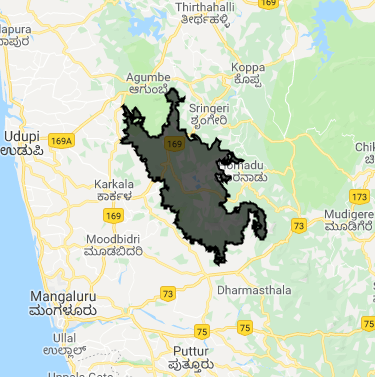
\includegraphics[width=0.5\linewidth, height=7cm]{geo.png} 
	%\caption{Caption1}
	\label{fig:subim1}
	\centering
	\caption{Geometry of the region}
\end{figure}

\begin{figure}{}
	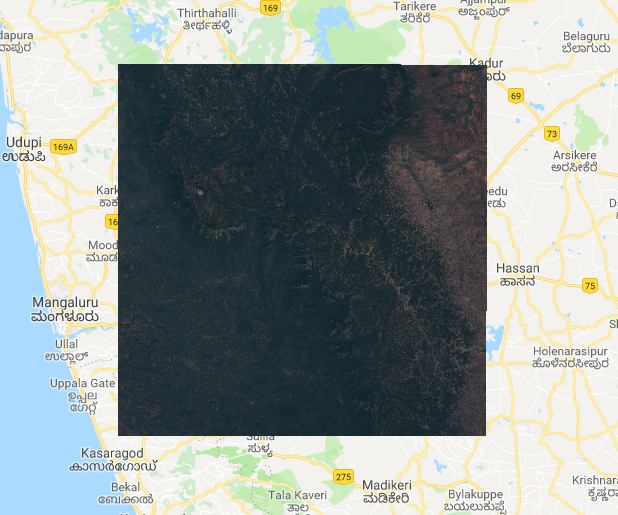
\includegraphics[width=0.6\linewidth, height=7cm]{prefire.png} 
	%\caption{Caption1}
	\label{fig:subim1}
	\centering
	\caption{Prefire RGB image}
\end{figure}

\begin{figure}{}
	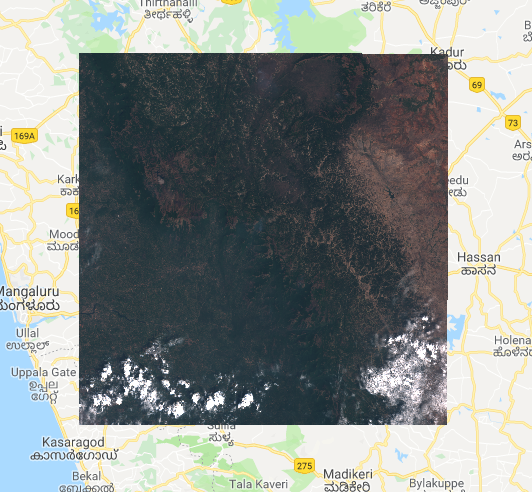
\includegraphics[width=0.6\linewidth, height=7cm]{postfire.png} 
	%\caption{Caption1}
	\label{fig:subim1}
	\centering
	\caption{Postfire Image}
\end{figure}

\begin{figure}{}
	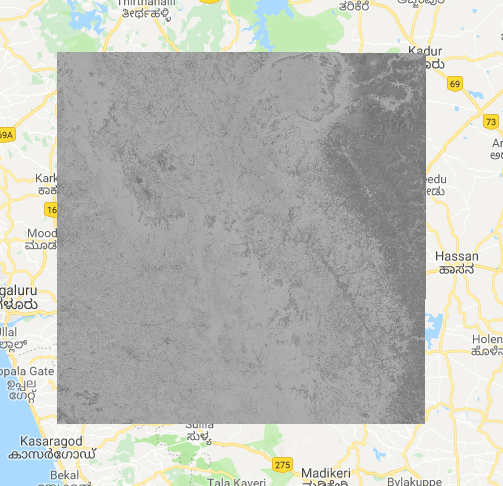
\includegraphics[width=0.6\linewidth, height=7cm]{prenbr.png} 
	%\caption{Caption1}
	\label{fig:subim1}
	\centering
	\caption{Prefire NBR}
\end{figure}

\begin{figure}{}
	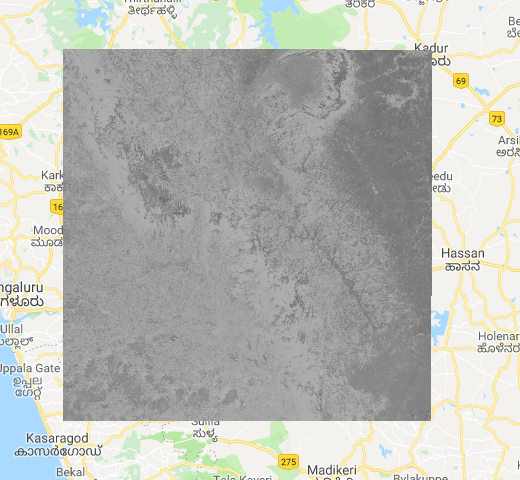
\includegraphics[width=0.6\linewidth, height=7cm]{postnbr.png} 
	%\caption{Caption1}
	\label{fig:subim1}
	\centering
	\caption{Postfire NBR}
\end{figure}

\begin{figure}{}
	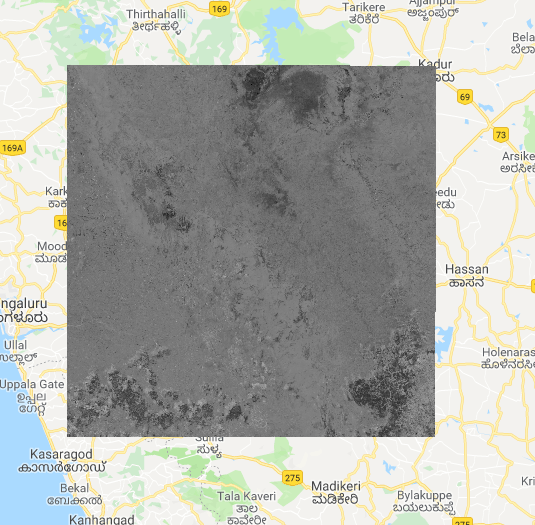
\includegraphics[width=0.6\linewidth, height=7cm]{dnbrnonclass.png} 
	%\caption{Caption1}
	\label{fig:subim1}
	\centering
	\caption{dNBR unclassified}
\end{figure}

\begin{figure}{}
	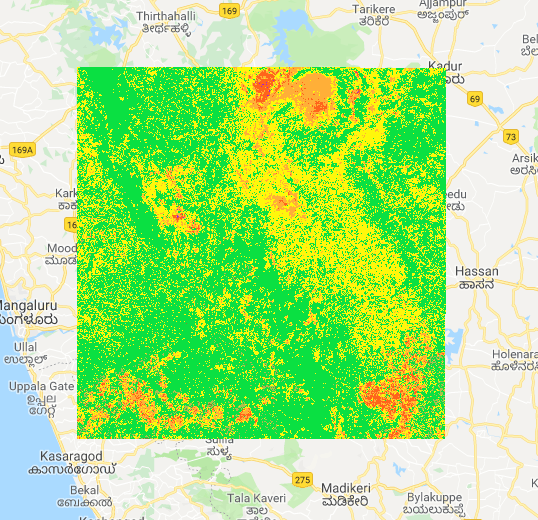
\includegraphics[width=0.6\linewidth, height=7cm]{dnbrclass.png} 
	%\caption{Caption1}
	\label{fig:subim1}
	\centering
	\caption{dNBR classified}
\end{figure}

\begin{figure}{}
	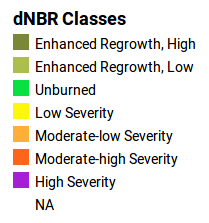
\includegraphics[width=0.5\linewidth, height=7cm]{classes.png} 
	%\caption{Caption1}
	\label{fig:subim1}
	\centering
	\caption{Classes made for segregation}
\end{figure}

\begin{figure}{}
	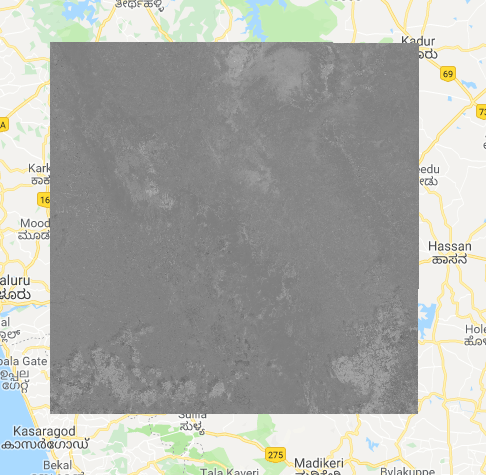
\includegraphics[width=0.6\linewidth, height=7cm]{delta.png} 
	%\caption{Caption1}
	\label{fig:subim1}
	\centering
	\caption{the dnbr grayscale original single band image}
\end{figure}

The above results are generated when the code is run. These images were exported and then checked using software and confirmed with the avilable data for firepoints. It was found that the firepoints matched exactly with the locations that were reported as burnt by the dnbr classification.\\

Very few of the points were shifted due to the image selected and the dates chosen as the fire might have shifted in that span from one point to another.




\subsection{Conclusion}



Earth Engine is not like any GIS you have ever used before! Because Earth Engine is a cloud-based platform, it is incredibly powerful. It is also strange and wondrous. The purpose of the docs in the How Earth Engine works section is to demystify some potentially surprising behavior you may encounter when running scripts in the Code Editor. This includes:

    Distinguishing between JavaScript objects in the client and Earth Engine objects on the server.
    The lazy computation model. 
    How Earth Engine handles scale (pixel resolution).
    How Earth Engine handles map projections.


\subsection{Acknowledgement}
I would like to acknowledge Ms. Amba Shetty for guiding me throughout the course of the project. Also, I would like to thank her for being a constant source of motivation for me to continue with this topic, which was a challenging and hard task.
I would also like to thank our faculty advisor, Ms. B R Jayalekshmi, for being supportive in proceeding with the course. 





\section{References}
\emph{
\begin{enumerate}
    \item https://developers.google.com/earth-engine/
    \item https://servirglobal.net/Portals/0/Documents/Articles/ChangeDetectionTraining/Modu\\le2\_Intro\_Google\_Earth\_Engine\_Exercise.pdf
    \item http://gsp.humboldt.edu/olm\_2015/Courses/GSP\_216\_Online/lesson5-1/NBR.html
    \item Bioucas-Dias, José M., et al. "Hyperspectral unmixing overview: Geometrical, statistical, and sparse regression-based approaches." IEEE journal of selected topics in applied earth observations and remote sensing 5.2 (2012): 354-379.
    \item Parra, Lucas C., Clay Spence, Paul Sajda, Andreas Ziehe, and Klaus-Robert Müller. "Unmixing hyperspectral data." In Advances in neural information processing systems, pp. 942-948. 2000.
    \item Drumetz, Lucas, et al. "Blind hyperspectral unmixing using an extended linear mixing model to address spectral variability." IEEE Transactions on Image Processing 25.8 (2016): 3890-3905.
    \item Code Source for the greedy sparse approximation algorithm:  (http://staffhome.ecm.uwa.ed\\u.au/~00053650/code.html)
    \item Sources: http://openremotesensing.net/knowledgebase/code-and-demo-for-hyperspectral-u\\nmixing-2
    \item Sources: http://openremotesensing.net/?s=Hyperspectral+Unmixing+Overview$\%$3A+Geome\\trical$\%$2C+Statistical$\%$2C+and+Sparse+Regression-Based+Approaches&post$_$type=
\end{enumerate}
}
%
% ---- Bibliography ----
%\bibliographystyle{apalike}
%\bibliography{my_library}

%deeparamesh88@yahoo.com
%title-application of greedy algorithhm for unmixing of hyperspectral data.
%conclsuion- how efficient algorithm is for the present dataset
\end{document}
